%======================================================================
% 2. ENTRY-VEHICLE MODEL AND VALIDATION
%======================================================================
\section{Entry-vehicle model and validation}
\label{sec:model}

\subsection{Geometry and parameterization}
\label{sec:geometry}

The vehicle is an axisymmetric capsule consisting of a spherical-section
forebody, a toroidal shoulder and a conical afterbody frustum
\cite{dirkx2017entry}. Three shape parameters are free: the nose radius
$R_n$, the shoulder radius $R_s$ and the afterbody cone half-angle
$\theta_c$. The maximum body radius ($R_m=\SI{2}{\metre}$) and the frustum
length ($L_c=\SI{2}{\metre}$) are held fixed, so the design space is
three-dimensional; Table~\ref{tab:bounds} lists the bounds. In the
optimizers the three variables are normalized to $[0,1]$.

Each shape carries its own mass through the Apollo-derived
constant-density model of \cite{dirkx2017entry}: the Apollo command module
($m=\SI{5470}{\kilogram}$, $V=\SI{20.02}{\cubic\metre}$) implies
$\rho=\SI{273.29}{\kilogram\per\cubic\metre}$, and $m=\rho V(\mathbf{x})$.
The centre-of-gravity placement follows the same Apollo-based offset model
and is not optimized. The first objective, volumetric efficiency
\begin{equation}
\eta_V \;=\; \frac{6\sqrt{\pi}\,V}{S^{3/2}} \;\in\; (0,1],
\label{eq:etav}
\end{equation}
equals unity for a sphere and rewards enclosed volume per wetted area; it
is an exact geometric quantity, evaluated from the shape and never
surrogated.

\begin{table}[htbp]
\centering
\caption{Design variables and fixed geometry.}
\label{tab:bounds}
\begin{tabular}{lccl}
\toprule
parameter & symbol & bounds & role \\
\midrule
nose radius            & $R_n$    & $3$--$7$ \si{\metre}          & free \\
shoulder radius        & $R_s$    & $0.02$--$0.4$ \si{\metre}     & free \\
afterbody half-angle   & $\theta_c$ & $5$--$60$ \si{\degree}      & free \\
max.\ body radius      & $R_m$    & $2$ \si{\metre} (fixed)       & fixed \\
afterbody length       & $L_c$    & $2$ \si{\metre} (fixed)       & fixed \\
\bottomrule
\end{tabular}
\end{table}

%% TODO figure (to build; thesis Fig 3.5 as template):
%% \begin{figure}[htbp]
%%   \centering\includegraphics[width=\linewidth]{fig_geometry_schematic}
%%   \caption{Capsule parameterization: spherical-section forebody
%%     (Rn), shoulder radius (Rs), afterbody cone half-angle (theta_c);
%%     local surface normal shown for the local-inclination method.}
%%   \label{fig:geometry}
%% \end{figure}

\subsection{Aerothermal model}
\label{sec:aero}

The atmosphere follows the U.S.\ Standard Atmosphere 1976 with the tabulated
86--120~km extension, interpolated between nodes \cite{us1976atmosphere};
above the homopause density is interpolated directly rather than recovered
from the gas law. Surface pressures come from a local-inclination method
\cite{dirkx2017entry,hirschel2009}: modified Newtonian on the windward
spherical nose,
an exact Taylor--Maccoll tangent-cone solution on the afterbody cone
(saturating to the Newtonian level beyond shock detachment), and
Prandtl--Meyer expansion on lee surfaces, with the cone and prism laws
Mach-blended over $M=5$--$12$ for continuity. Integrating the local
coefficients over the meridional contour yields $C_D$, $C_L$ and $C_m$
databases on a grid of $M\in[3,30]$ (ten nodes) and
$\alpha\in[-5^\circ,35^\circ]$ (41 nodes); bivariate interpolation supplies
forces and moments in flight. The trim angle of attack solves $C_m=0$ at
each Mach number, and the trajectory flies at trim.

Stagnation-point convective heating uses the Sutton--Graves form of the
$\sqrt{\rho}\,V^3$ correlation \cite{sutton1971}
with the effective nose radius $R_{\mathrm{eff}}$ of Zoby and Sullivan
\cite{zoby1965heating}, read from their chart for the actual
$(R_m/R_n,\,R_s/R_m)$ combination; the in-code chart reproduces the
published curves to within 1.4\% over the design space. Shoulder heating is
taken as a correlated fraction of the stagnation value through a linear
relation in Mach number, angle of attack, $R_s/R_m$ and the nose-sphere
half-angle, fitted to wind-tunnel measurements of the shoulder-to-stagnation
ratio; the fit reproduces the source ratios to within 10.2\% and inherits
their trends (rising with $\alpha$, falling with $R_s$). A cold wall
($T_w/T_{aw}=0$) is assumed throughout.

\subsection{Trajectory simulation}
\label{sec:traj}

Entry is propagated with a point-mass three-degree-of-freedom model over a
spherical, rotating Earth, in the ballistic-entry tradition of Allen and
Eggers \cite{allen1958} as formalized for entry mechanics by Vinh et al.\
\cite{vinh1980}. The state is
$(h,V,\gamma,\varphi,\lambda,\chi,\sigma)$; the bank angle $\sigma$ is a
propagated seventh state that tracks the no-skip bank command of
\cite{dirkx2017entry} through a first-order lag capped at
\SI{5}{\degree\per\s}, which removes the on/off chatter of the idealized
command and mirrors the finite roll rate of a real vehicle. The modulation
is active only while $0<\cos\sigma<1$; outside that band the vehicle flies
full lift-up. Integration uses an adaptive Runge--Kutta scheme and
terminates at $M=3$, with a horizon of $t_{\max}=\SI{14400}{\s}$ (the
horizon was raised from an initial 7{,}200~s during data-quality auditing;
Section~\ref{sec:doe}).

Each run returns five quantities: the integrated stagnation heat load
$Q_s=\int q_{\mathrm{stag}}\,dt$; the range $sg$, defined as the
great-circle distance between the entry-interface position and the final
position (a lower bound on ground-track length, with a physical maximum of
$\pi R_{\oplus}\approx\SI{20015}{\kilo\metre}$); the peak stagnation and
shoulder heat fluxes; and the peak load factor. The load-factor metric is
drag-based, $n_D=D/(mg)$; the total-force definition
$n=\sqrt{D^2+L^2}/(mg)=n_D\sqrt{1+(L/D)^2}$ exceeds it by 4--5\% at capsule
lift-to-drag ratios, and both are reported where the distinction matters.

\subsection{Validation against reference data}
\label{sec:validation}

The chain was validated layer by layer against Dirkx and Mooij
\cite{dirkx2017entry}, whose reference figures were digitized (per-subpanel
calibration; tracing artifacts removed by a documented filter, with all
verdicts re-checked for stability); the full audit, including the
reference-data forensics summarized below, is reproduced in
Appendix~\ref{app:validation}. Component-level verification against
analytic benchmarks (Taylor--Maccoll against exact cone solutions,
Prandtl--Meyer against published anchor angles, atmosphere against
standard tables) precedes any comparison with the reference mission, so
equation and implementation errors are separated from mission-level
agreement throughout. The atmosphere reproduces the standard
anchor values to $2\times10^{-5}$ relative. The surface-pressure laws match
the book's correlation charts to within 0.026~$C_p$ (modified Newtonian) and
0.061~$C_p$ (tangent-cone core, $M=3$, against a 0.065 band attributable to
the documented beyond-detachment treatment). The core aerodynamic check
compares Apollo force coefficients at $M=3$ and $M=10$ against wind-tunnel
data as re-plotted by Dirkx and Mooij (originally from the stability test
campaign of NASA TN D-3890 \cite{moseley1967d3890}, with the flight and
tunnel data bases of \cite{hillje1969apollo,moseley1969wind}): nine of nine
checks pass,
lift-to-drag ratio to within 0.029 absolute and the coefficient shapes to
within 0.015 after scale removal. The known over-prediction of
$C_D(\alpha\approx0)$ at $M=10$ inherent to local-inclination methods lands
at 1.610 against a wind-tunnel value of 1.523 --- between the tunnel and the
book's own implementation (1.704). The heating model reproduces the
Zoby--Sullivan chart to 1.4\%, the shoulder-ratio sources to 10.2\%, and the
computed trim angles match the reference trim curve to 0.33$^\circ$.

On the full Apollo entry case ($V_0=7.83$~km/s, $\gamma_0=-4^\circ$,
$m=4532$~kg, the reference initial conditions), the implementation
reproduces the published peak heat rate to 0.7\%; integrated heat load and
track length sit $+32\%$ and $+16\%$ above the reference table. The
end-to-end differences are bounded and attributed rather than resolved:
they concentrate in the guidance realization and in the reference data
themselves. Panel~(c) of the reference Fig.~7.17 plots $\dot{q}(M)$ and
$n(M)$ for one simulation; these quantities are algebraically coupled
independent of trajectory model, and the digitized pair violates that
identity by factors of 0.17--0.65, so the load-factor panel is not a valid
target --- and the reference table itself lies below every member of a
documented variant family of the bank law whose digitized $\dot{q}$ curve
runs above ours (Appendix~\ref{app:variants}). Within that family, peak
heat rate and track length are individually reproducible to 0.7\% and
$-1.1\%$, and no member reproduces the table and the panels
simultaneously; the family floor for integrated heat load is $+16\%$. The
deviations between the present implementation and the reference --- the
bank-rate limit, the Prandtl--Meyer lee treatment, the omission of base
pressure, the Mach-grid extension to 30, and the moment-reference and
load-factor conventions --- are each quantified in
Appendix~\ref{app:deviations}. In short, the model is
\emph{component-validated} at the percent level, with end-to-end
discrepancies against the single available reference case attributed to
specific, documented causes; the residual force-level model-form error is
what the uncertainty model of Section~\ref{sec:surrogate} represents.

Which of this paper's claims depend on that residual absolute accuracy is
therefore worth stating once, explicitly, as three claims of different
strength. (i)~\emph{The component models reproduce their analytical and
reference benchmarks}: supported at the percent level above. (ii)~\emph{The
complete simulator produces credible predictions for this entry
scenario}: partially supported --- peak heat rate reproduces the only
end-to-end reference to 0.7\%, while integrated heat load and track length
sit $+32\%$/$+16\%$ above a reference table that is itself internally
inconsistent; the discrepancies are bounded and attributed
(Appendix~\ref{app:validation}), not resolved. (iii)~\emph{The relative
comparison between the two formulations is reliable}: supported by
construction --- every comparison runs on one simulator, one surrogate,
and one common-random-number lens, so shared model error cancels to first
order --- and by simulator-level verification
(Section~\ref{sec:verification}). The paper's conclusions rest on (i)
and (iii); (ii) bounds the absolute meaning of objective values and of
the constraint-boundary positions (the 5-$g$ and heat-flux limits bind
against aerodynamics whose absolute level carries the attributed offset),
not the comparisons themselves. The sensitivity studies of
Sections~\ref{sec:surrogate} and \ref{sec:sens} additionally probe the
reported statistics against changes in the uncertainty model itself.

\begin{figure}[htbp]
\centering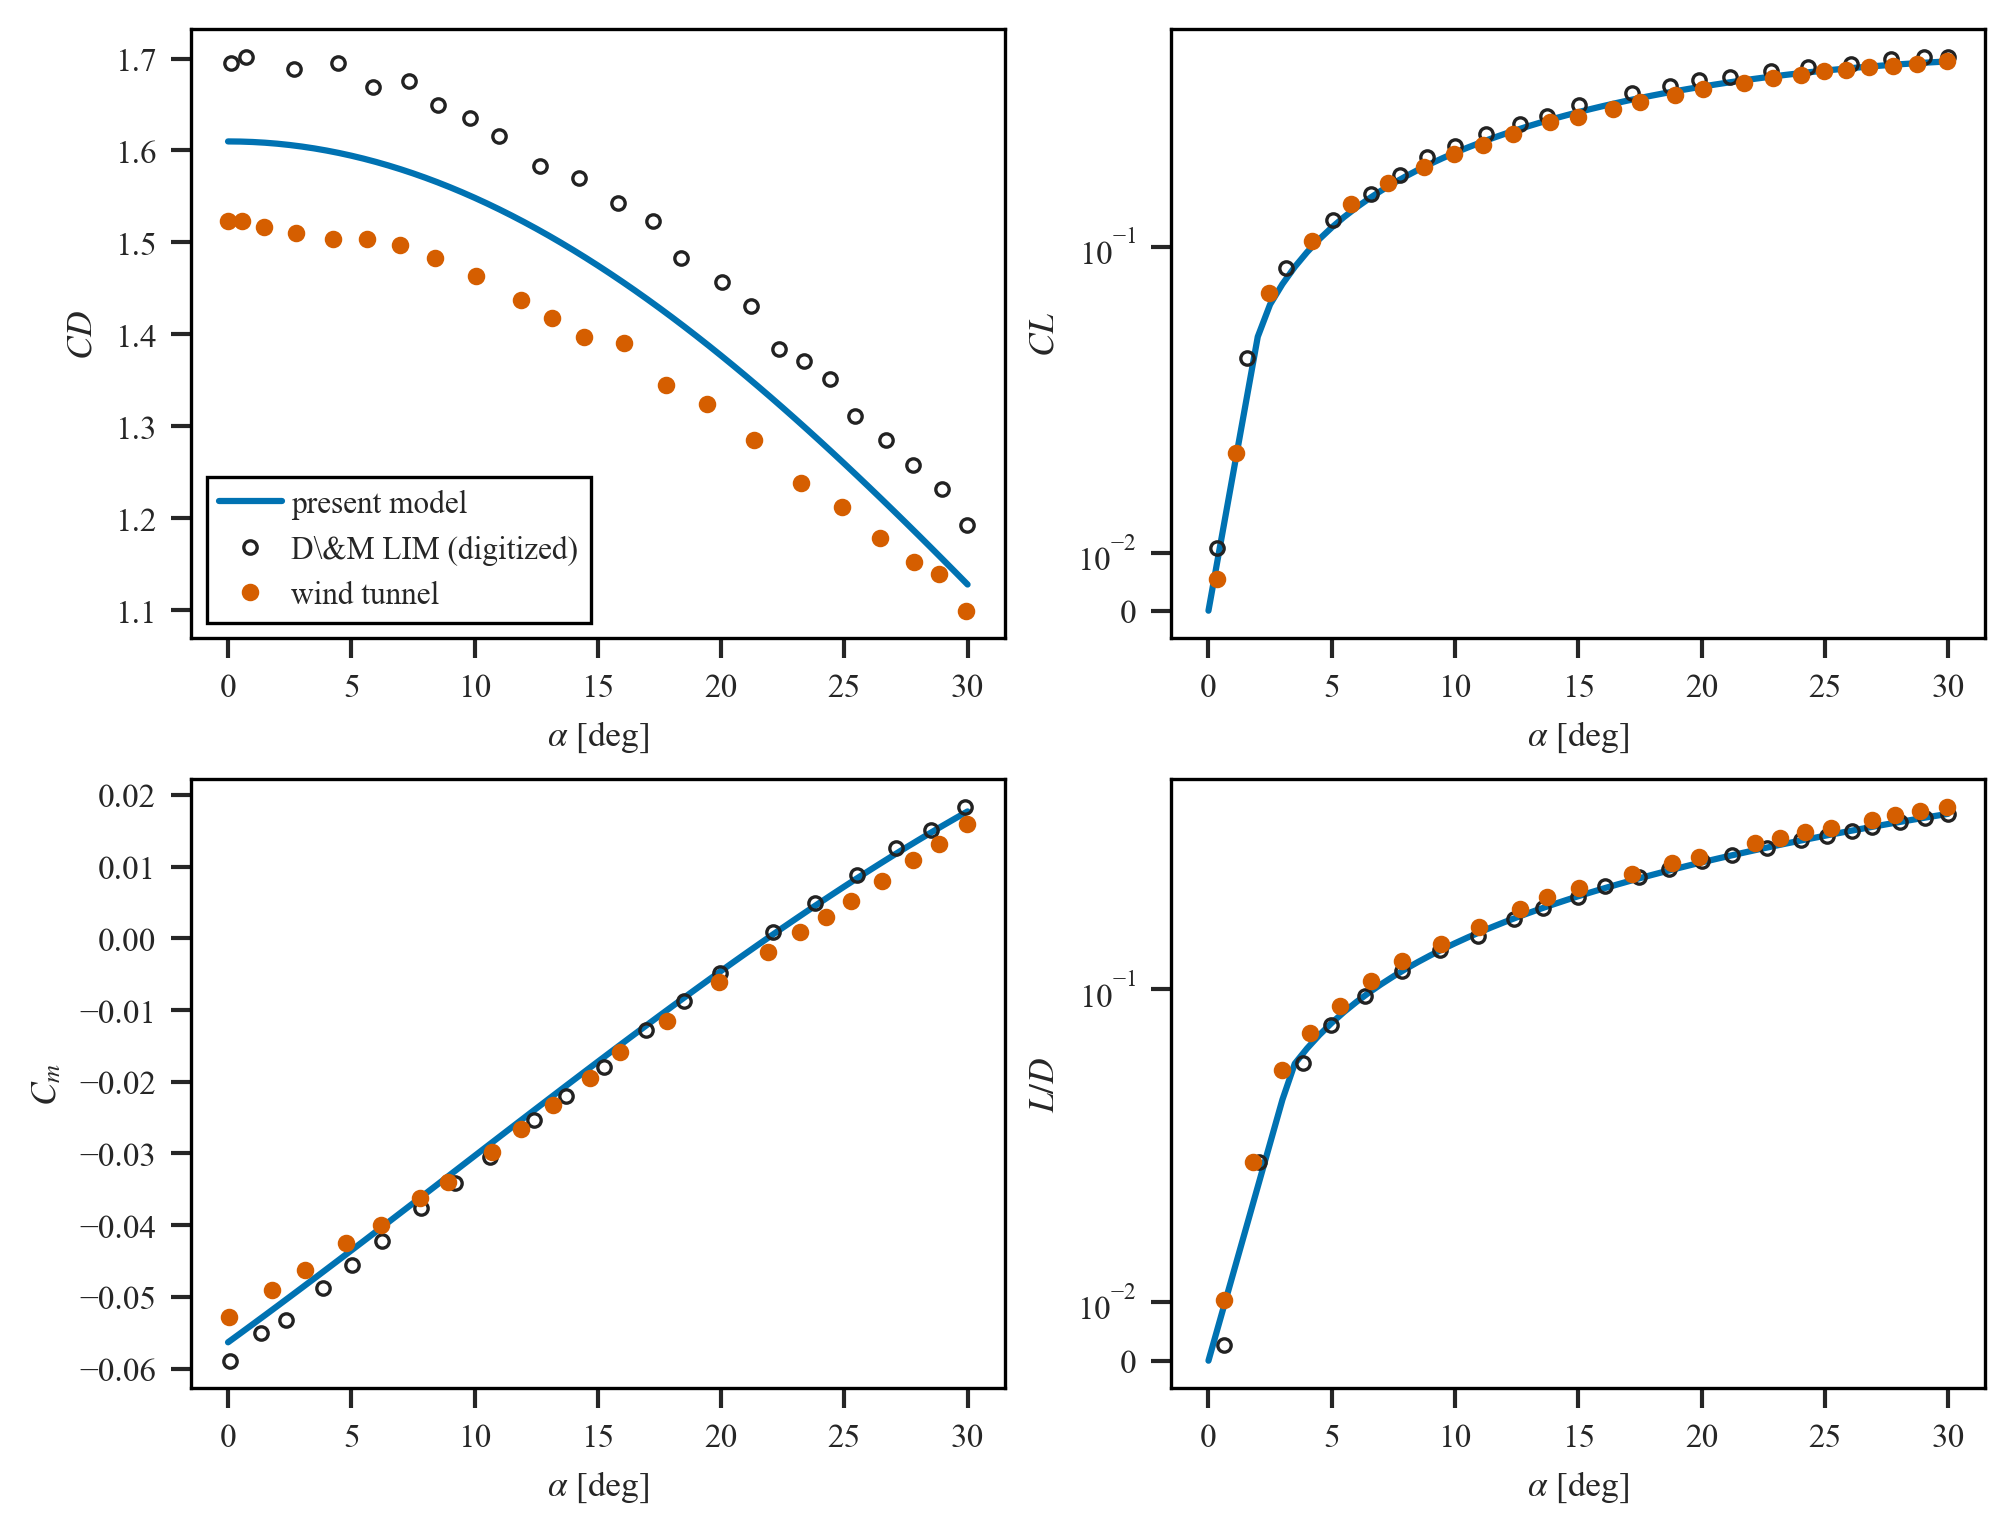
\includegraphics[width=\linewidth]{fig_validation_aero}
\caption{Apollo force coefficients at $M=10$: present local-inclination
  model (line), the digitized local-inclination curves of the reference
  (circles), and wind-tunnel data (crosses), in the present model's
  angle-of-attack sign convention. Lift-to-drag agrees to within 0.007
  absolute; the known local-inclination over-prediction of
  $C_D(\alpha\approx0)$ places the present model (1.610) between the
  tunnel (1.523) and the reference implementation (1.704). The $M=3$
  counterpart is Fig.~S2 (supplementary material).}
\label{fig:v2aero}
\end{figure}

\begin{figure}[htbp]
\centering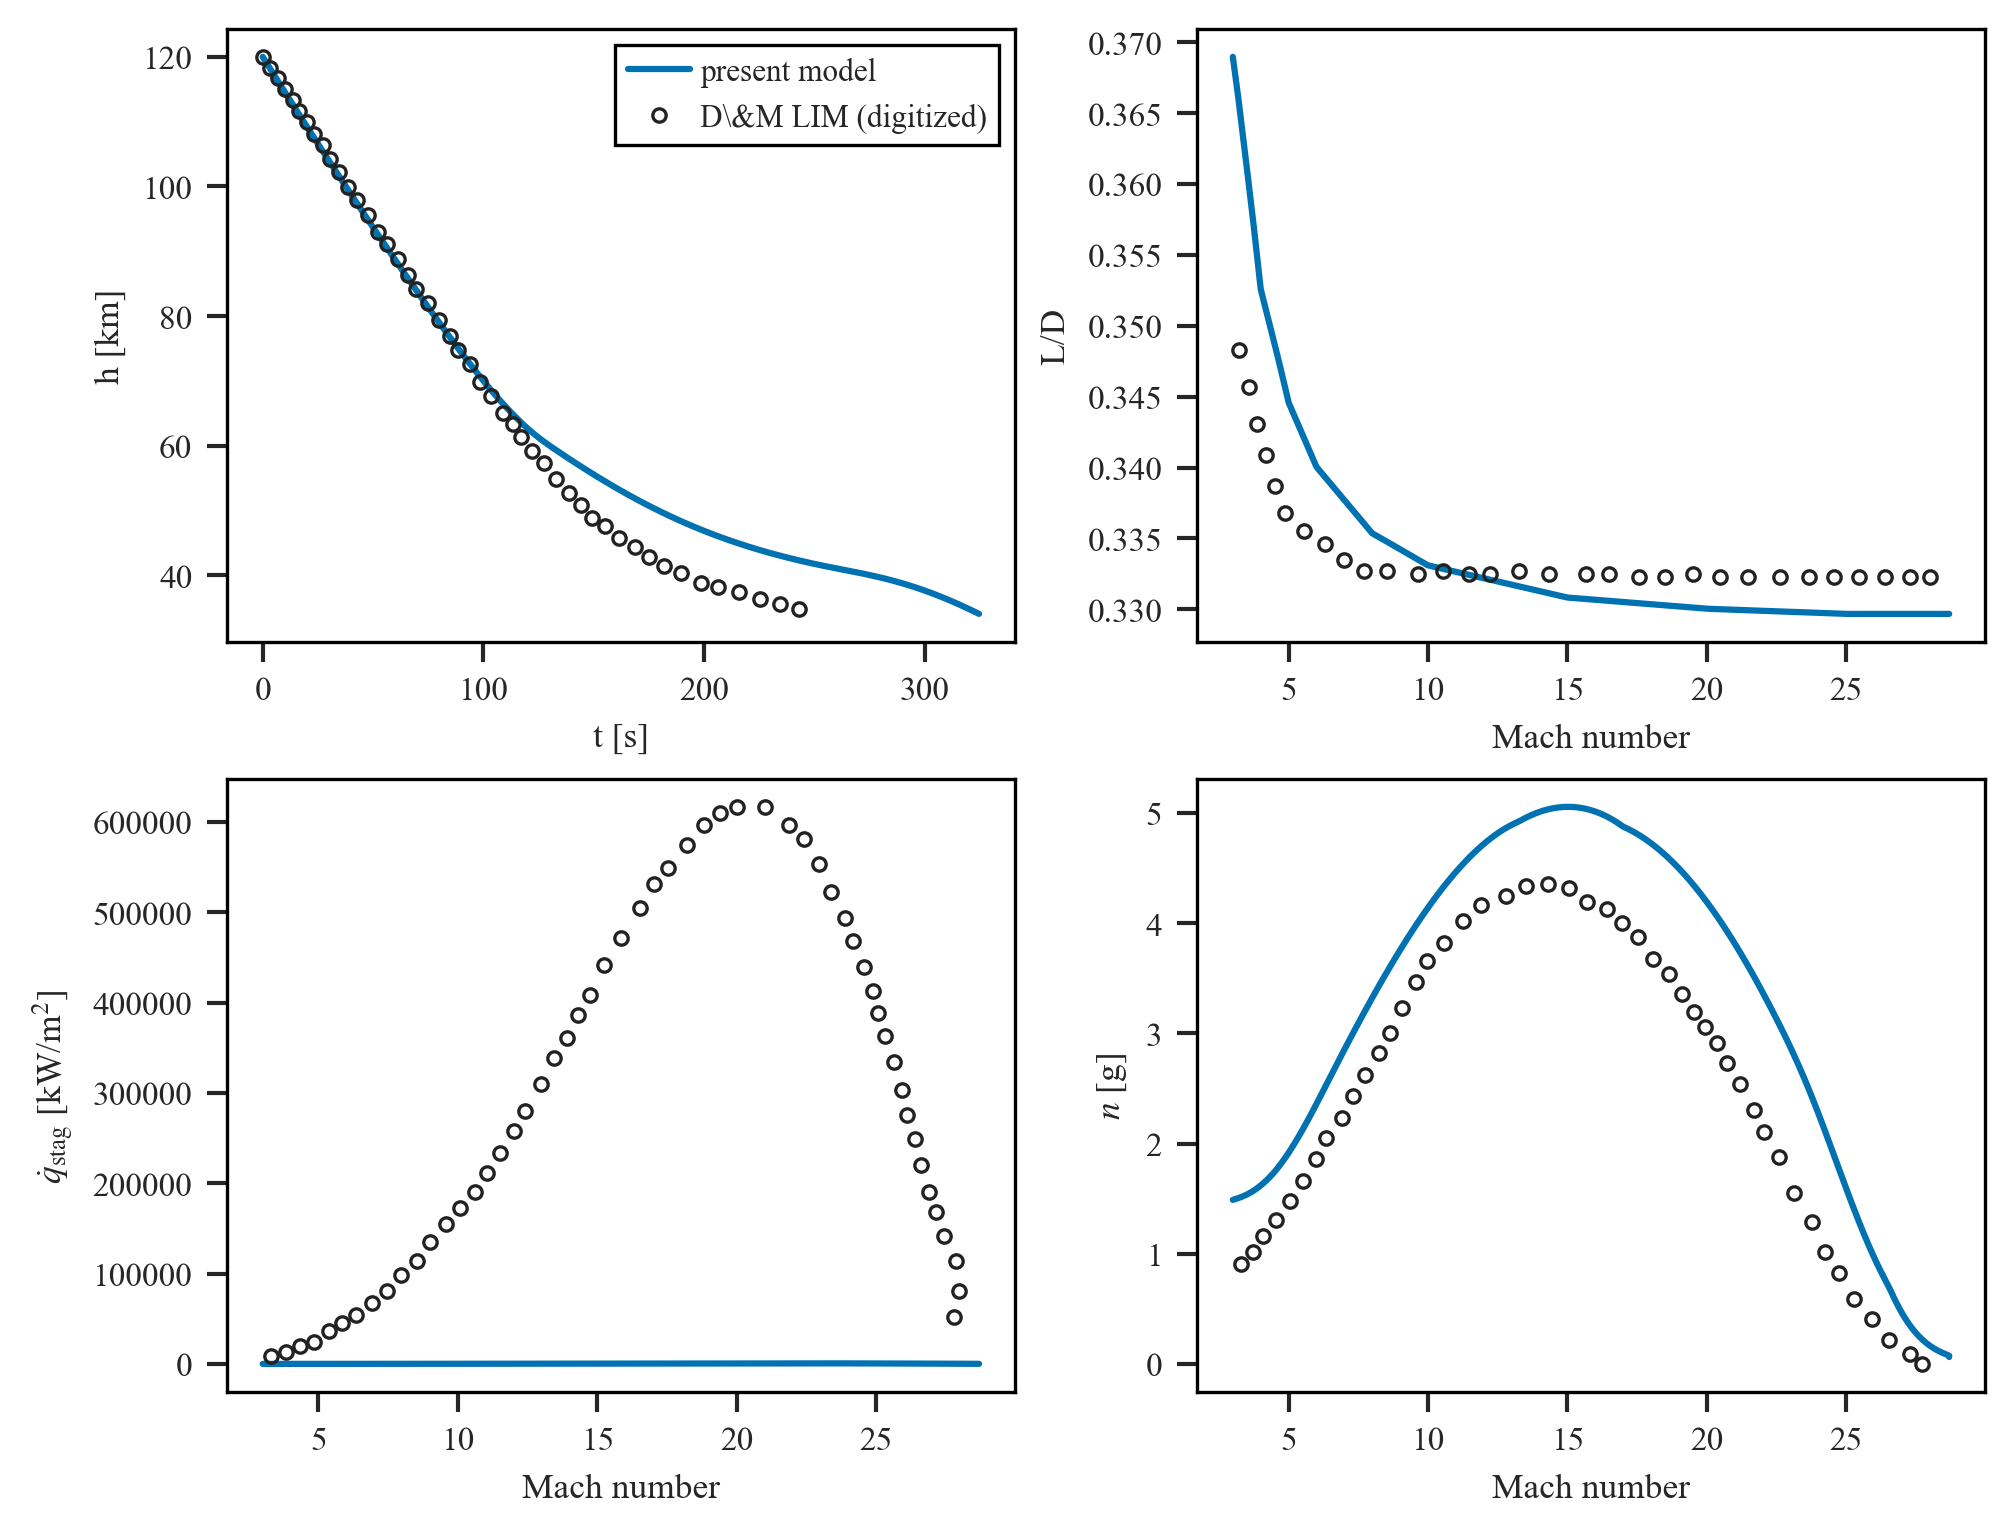
\includegraphics[width=\linewidth]{fig_validation_traj}
\caption{Apollo entry case ($V_0=7.83$~km/s, $\gamma_0=-4^\circ$,
  $m=4532$~kg): altitude, lift-to-drag ratio, stagnation heat rate, and
  load factor from the present model (lines) against the digitized
  reference profiles (circles). Peak heat rate reproduces the reference
  to 0.7\%; the load-factor panel is qualitative only, per the reference
  inconsistency documented in Appendix~\ref{app:identity}.}
\label{fig:v4traj}
\end{figure}

\begin{figure}[htbp]
\centering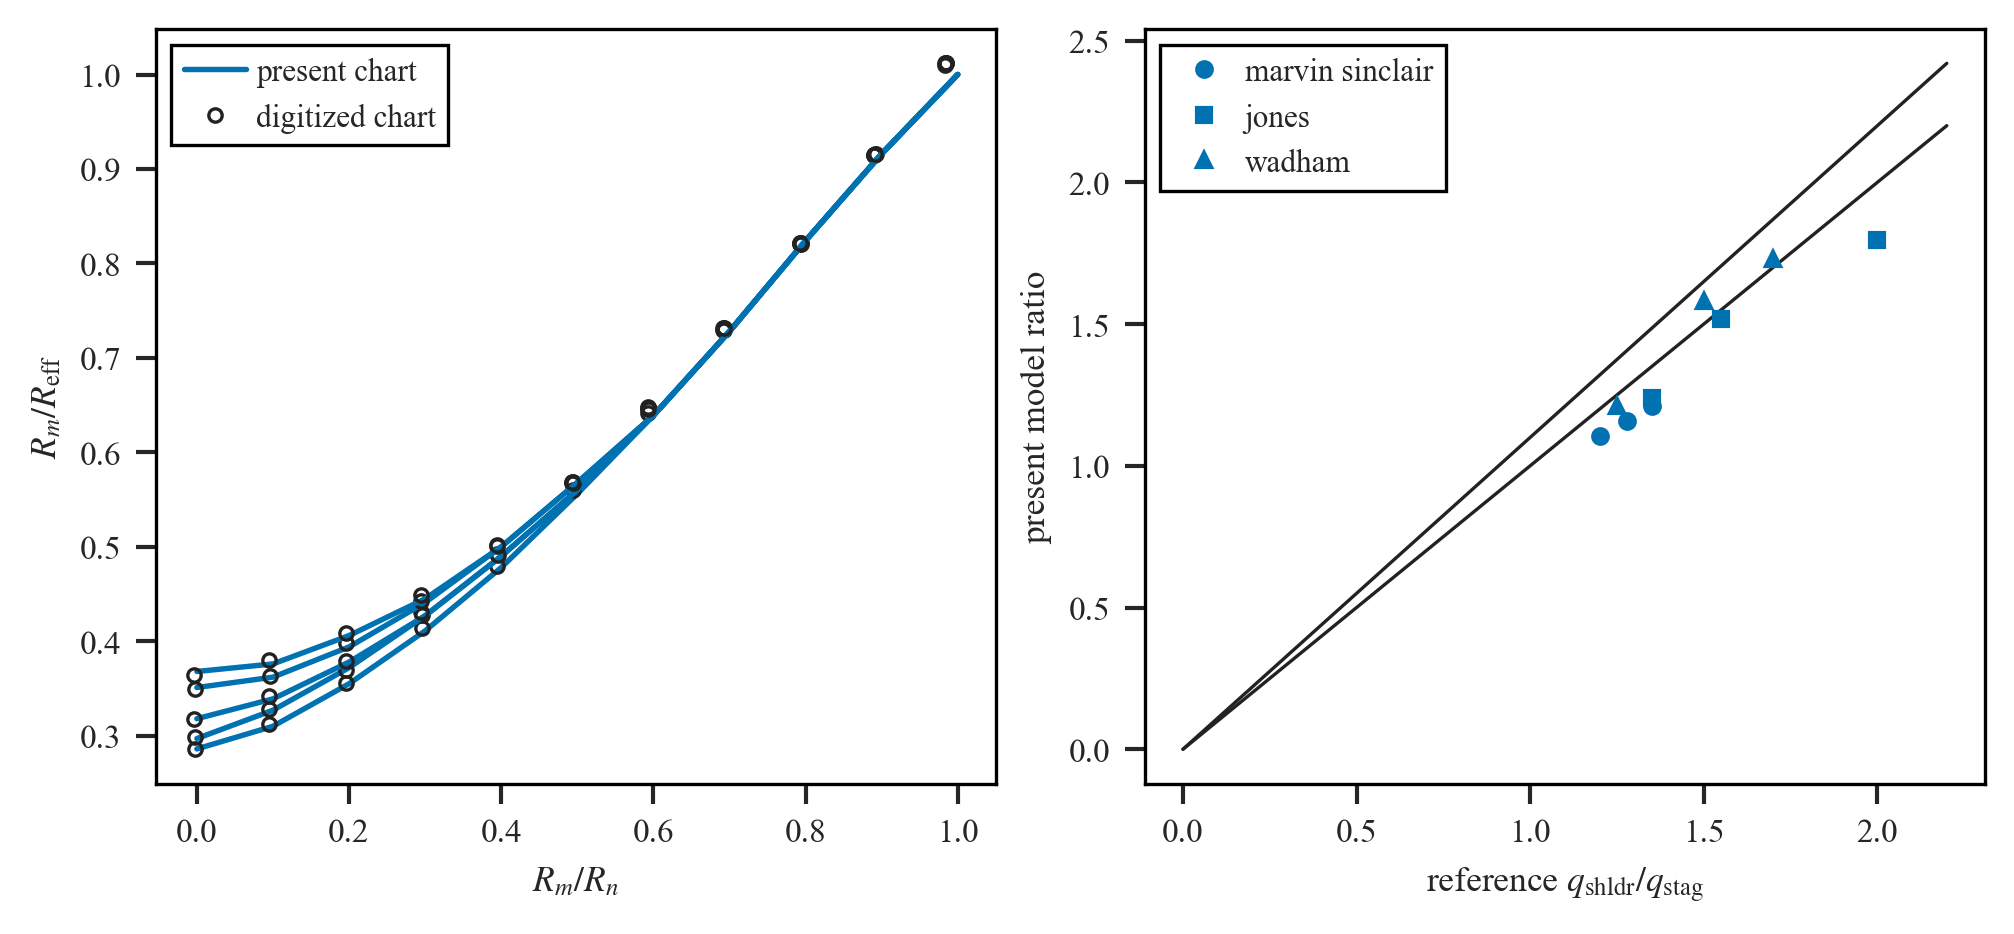
\includegraphics[width=\linewidth]{fig_validation_heating}
\caption{Heating-model validation. (a) Zoby--Sullivan effective
  nose-radius chart: present interpolation (lines) against the digitized
  chart (circles) for five shoulder-to-body radius ratios, agreement
  within 0.014 over the design-space region ($R_m/R_n\le0.7$). (b)
  Shoulder-to-stagnation heat-flux ratio: present correlation against
  the wind-tunnel source measurements, worst deviation 10.2\%.}
\label{fig:v3heat}
\end{figure}
